\documentclass[10.5pt,journal, a4paper]{IEEEtran}

\makeatletter
\newcommand\subparagraph{%
  \@startsection{subparagraph}{5}
  {\parindent}
  {3.25ex \@plus 1ex \@minus .2ex}
  {-1em}
  {\normalfont\normalsize\bfseries}}
\makeatother
\usepackage{titlesec}
\let\subparagraph\relax % You don't want to use \subparagraph

% some very useful LaTeX packages include:

%\usepackage{cite}      % Written by Donald Arseneau
                        % V1.6 and later of IEEEtran pre-defines the format
                        % of the cite.sty package \cite{} output to follow
                        % that of IEEE. Loading the cite package will
                        % result in citation numbers being automatically
                        % sorted and properly "ranged". i.e.,
                        % [1], [9], [2], [7], [5], [6]
                        % (without using cite.sty)
                        % will become:
                        % [1], [2], [5]--[7], [9] (using cite.sty)
                        % cite.sty's \cite will automatically add leading
                        % space, if needed. Use cite.sty's noadjust option
                        % (cite.sty V3.8 and later) if you want to turn this
                        % off. cite.sty is already installed on most LaTeX
                        % systems. The latest version can be obtained at:
                        % http://www.ctan.org/tex-archive/macros/latex/contrib/supported/cite/
\usepackage{float}
\usepackage{graphicx}   % Written by David Carlisle and Sebastian Rahtz
                        % Required if you want graphics, photos, etc.
                        % graphicx.sty is already installed on most LaTeX
                        % systems. The latest version and documentation can
                        % be obtained at:
                        % http://www.ctan.org/tex-archive/macros/latex/required/graphics/
                        % Another good source of documentation is "Using
                        % Imported Graphics in LaTeX2e" by Keith Reckdahl
                        % which can be found as esplatex.ps and epslatex.pdf
                        % at: http://www.ctan.org/tex-archive/info/


%\usepackage{psfrag}    % Written by Craig Barratt, Michael C. Grant,
                        % and David Carlisle
                        % This package allows you to substitute LaTeX
                        % commands for text in imported EPS graphic files.
                        % In this way, LaTeX symbols can be placed into
                        % graphics that have been generated by other
                        % applications. You must use latex->dvips->ps2pdf
                        % workflow (not direct pdf output from pdflatex) if
                        % you wish to use this capability because it works
                        % via some PostScript tricks. Alternatively, the
                        % graphics could be processed as separate files via
                        % psfrag and dvips, then converted to PDF for
                        % inclusion in the main file which uses pdflatex.
                        % Docs are in "The PSfrag System" by Michael C. Grant
                        % and David Carlisle. There is also some information
                        % about using psfrag in "Using Imported Graphics in
                        % LaTeX2e" by Keith Reckdahl which documents the
                        % graphicx package (see above). The psfrag package
                        % and documentation can be obtained at:
                        % http://www.ctan.org/tex-archive/macros/latex/contrib/supported/psfrag/

%\usepackage{subfigure} % Written by Steven Douglas Cochran
                        % This package makes it easy to put subfigures
                        % in your figures. i.e., "figure 1a and 1b"
                        % Docs are in "Using Imported Graphics in LaTeX2e"
                        % by Keith Reckdahl which also documents the graphicx
                        % package (see above). subfigure.sty is already
                        % installed on most LaTeX systems. The latest version
                        % and documentation can be obtained at:
                        % http://www.ctan.org/tex-archive/macros/latex/contrib/supported/subfigure/

\usepackage{url}        % Written by Donald Arseneau
                        % Provides better support for handling and breaking
                        % URLs. url.sty is already installed on most LaTeX
                        % systems. The latest version can be obtained at:
                        % http://www.ctan.org/tex-archive/macros/latex/contrib/other/misc/
                        % Read the url.sty source comments for usage information.

%\usepackage{stfloats}  % Written by Sigitas Tolusis
                        % Gives LaTeX2e the ability to do double column
                        % floats at the bottom of the page as well as the top.
                        % (e.g., "\begin{figure*}[!b]" is not normally
                        % possible in LaTeX2e). This is an invasive package
                        % which rewrites many portions of the LaTeX2e output
                        % routines. It may not work with other packages that
                        % modify the LaTeX2e output routine and/or with other
                        % versions of LaTeX. The latest version and
                        % documentation can be obtained at:
                        % http://www.ctan.org/tex-archive/macros/latex/contrib/supported/sttools/
                        % Documentation is contained in the stfloats.sty
                        % comments as well as in the presfull.pdf file.
                        % Do not use the stfloats baselinefloat ability as
                        % IEEE does not allow \baselineskip to stretch.
                        % Authors submitting work to the IEEE should note
                        % that IEEE rarely uses double column equations and
                        % that authors should try to avoid such use.
                        % Do not be tempted to use the cuted.sty or
                        % midfloat.sty package (by the same author) as IEEE
                        % does not format its papers in such ways.



\usepackage{amsmath}  
\usepackage{lettrine}
\usepackage{titlesec}
\usepackage{graphics}
\usepackage{ragged2e}
\usepackage{multicol}
\usepackage[linesnumbered,ruled]{algorithm2e}
%\usepackage{titlesec} % From the American Mathematical Society
                        % A popular package that provides many helpful commands
                        % for dealing with mathematics. Note that the AMSmath
                        % package sets \interdisplaylinepenalty to 10000 thus
                        % preventing page breaks from occurring within multiline
                        % equations. Use:
%\interdisplaylinepenalty=2500
                        % after loading amsmath to restore such page breaks
                        % as IEEEtran.cls normally does. amsmath.sty is already
                        % installed on most LaTeX systems. The latest version
                        % and documentation can be obtained at:
                        % http://www.ctan.org/tex-archive/macros/latex/required/amslatex/math/
\usepackage{listings}
\lstset{breaklines=true}

% Other popular packages for formatting tables and equations include:

%\usepackage{array}
% Frank Mittelbach's and David Carlisle's array.sty which improves the
% LaTeX2e array and tabular environments to provide better appearances and
% additional user controls. array.sty is already installed on most systems.
% The latest version and documentation can be obtained at:
% http://www.ctan.org/tex-archive/macros/latex/required/tools/

% V1.6 of IEEEtran contains the IEEEeqnarray family of commands that can
% be used to generate multiline equations as well as matrices, tables, etc.

% Also of notable interest:
% Scott Pakin's eqparbox package for creating (automatically sized) equal
% width boxes. Available:
% http://www.ctan.org/tex-archive/macros/latex/contrib/supported/eqparbox/

% *** Do not adjust lengths that control margins, column widths, etc. ***
% *** Do not use packages that alter fonts (such as pslatex).         ***
% There should be no need to do such things with IEEEtran.cls V1.6 and later.
%\titlespacing\section{0pt}{2pt plus 4pt minus 2pt}{2pt plus 2pt minus 2pt}
%\titlespacing\subsection{0pt}{2pt plus 4pt minus 2pt}{0pt plus 2pt minus 2pt}
%\titlespacing\subsubsection{0pt}{0pt plus 4pt minus 2pt}{0pt plus 2pt minus 2pt}

%\titlespacing\author{0pt}{0pt minus 12pt minus 8pt}{0pt minus 12pt minus 8pt}

%\titlespacing\abstract{0pt}{0pt minus 100pt minus 20pt}{0pt minus 40pt minus 40pt}

% Your document starts here!
\title{\LARGE {Software  Analysis Using Code Metrics}}
\author{\small {Darren Blanckensee | 1147279}}



\begin{document}

% Define document title and author
	
%	\thanks{Advisor: Dipl.--Ing.~Firstname Lastname, Lehrstuhl f\"ur Nachrichtentechnik, TUM, WS 2050/2051.
%}
	\markboth{University of Witwatersrand}{}
	\maketitle

% Write abstract here

\begin{abstract}

\end{abstract}


% Each section begins with a \section{title} command

\section{Introduction}
\noindent
\IEEEPARstart{S}{oftware} is being developed at an ever increasing rate. It is important when writing programs to follow good programming practices and to hold the code one writes to a certain standard so as to ensure a high quality product. Often when software projects are large with many different classes and files with thousands of lines to keep track of it becomes increasingly difficult to maintain a standard as it becomes impossible for developers to read all the lines of code and make sure that the quality requirements are met. One way to address this issue is to make use of software metrics. Software metrics are standards of measurement that provide developers with quantifiable measurements of various characteristics of the code they have developed. \\

\noindent
One of the most simple metrics often used as an example in software is the lines of code metric (LOC) which measures how many lines of code exist in a program. This metric alone does not however provide the developer with useful information relating to the quality of the software and whether or not good programming practices are being followed. As So and so once said Puthequoteherepleasedarren. Other more useful metrics exist and the use of these in analysing software projects is the purpose of this report. All code in this project (including the metrics tool used) is written in Python.  \\

\noindent
The Chosen Metrics section details which metrics have been selected to allow for sound analysis of a code base that provides developers with useful information that could be used to maintain a standard of coding. Along with the selected metrics, explanations of each metric will be provided so as to explain the importance of each of the chosen metrics and how they should be used. The Code Base Analysis section covers the analysis of the authors own code base along with three major releases of the open source software, Freevo Media Library. 



\section{Understanding Chosen Metrics}
\noindent
The metrics being used in this project are the following:
\begin{itemize}
\item Cyclomatic Complexity
\item Maintainability Index
\item Coverage
\item Halstead Metrics
\item Dependencies
\end{itemize}
\noindent
The tools used to calculate these metrics are Radon, Pylint, Graphviz, Webdot and Snakefood. Each of these metrics used are explained in the subsections below.

\subsection{Cyclomatic Complexity}
\noindent
The cyclomatic complexity metric, calculated using the Radon tool, is used to determine the number of distinct paths a program can take during running. It gives the developer an idea of how many decisions are being made by their code. There are various constructs and conditional statements or decisions that have an effect on the cyclomatic complexity of any program. These and their additive  effects on the cyclomatic complexity are shown in the table below. 

\begin{table}[H]
\centering
\caption{Statements and their effects on cyclomatic complexity}
\label{my-label}
\begin{tabular}{|l|l|}
\hline
Statement         & Effect On Cyclomatic Complexity \\ \hline
If                & 1                               \\ \hline
Elif              & 1                               \\ \hline
Else              & 0                               \\ \hline
For               & 1                               \\ \hline
While             & 1                               \\ \hline
Except            & 1                               \\ \hline
Finally           & 0                               \\ \hline
With              & 1                               \\ \hline
Assert            & 1                               \\ \hline
Comprehension     & 1                               \\ \hline
Boolean Operators & 1                               \\ \hline
\end{tabular}
\end{table}

\noindent
An example (not the author's code base) and its cyclomatic complexity are shown in figure 1 and the paragraph that follows respectively. 


\lstinputlisting[caption=Example code to explain cyclomatic complexity metric.,language=python]{dog.py}

\noindent
While this code is simple and may not follow the best programming practices it is sufficient to explain how the cyclomatic complexity metric works. There are four ways this code can run. The first being if the dog is hungry and it is home then the dog will be fed. The second being if the dog is hungry but is not home then the dog will be located and fed. The third way is if the dog is not hungry and is not home then the dog will be located. The last way is if the dog is not hungry but is home then nothing is to be done. Because there are four ways this program can be run the cyclomatic complexity of this code is 4.\\  



\noindent
Radon was used to calculate the cyclomatic complexity of the various code bases analysed in this project. Radon's cyclomatic complexity measurement outputs a letter between A and F along with a score larger than zero relating to the number of decisions. A relates to a section of code that has less than five decisions while F relates to more than 41 decisions. The scores and letters are produced for each class, method and function.\\

\noindent
The cyclomatic complexity command on Radon returns these letters and scores for each class, method and function in a section of code. Code with many decisions means many different ways the code can run which leads to high risk that code may not behave as the developer expects or intends. It is ideal to have a cyclomatic complexity score of less than 10 or B \cite{mcCabe}.  


\subsection{Maintainability Index}
\noindent
The maintainability index, calculated using the Radon tool, is used to determine how easily a section of code can be maintained. This metric measures how easy it would be to change this code in future. The maintainability index as a metric was introduced is calculated using the equation below. 


\begin{equation}
\resizebox{0.5\textwidth}{!}{ $MI = \emph{max} [0,100*\frac{171-5.2\ln\emph{V}-0.23\emph{G} -16.2\ln\emph{L} + 50\sin(\sqrt{2.4\emph{C}}) }{171}]$}
\end{equation}
Where V is the Halstead volume, G is cyclomatic complexity, L is the number of source lines of code and C is the percent of comment lines in the program converted to radians. This equation is Radon's variation from the original maintainability index formula. In \cite{MI1} Coleman et al. using a slightly different equation state that a maintainability index of above 85 is ideal and relates to code that is easy to maintain and update, while code with a maintainability index of between 85 and 65 is fairly maintainable and a maintainability index of less than 65 relates to code that is very difficult to maintain. Translating these values generated from the formula used in \cite{MI1} to values generated from the formula in equation 1 above (used by Radon); A value of 85 and above using Coleman's formula corresponds to a value of 20 and above, a value of between 85 and 65 using Coleman's formula corresponds to a values between 20 and 10 and a value of below 65 using Coleman's formula corresponds to a value below 10. \\

\noindent
For programs that are long term and will have many releases this metric is very important as it helps developers ensure that their code is written in a way that allows it to be changed and improved easily. This will help developers in the future tasked with working on that code perhaps to add new features or fix bugs. In \cite{Linux} various versions of the Linux kernel are analysed using the maintainability index and it can be seen that with each new release the maintainability index actually increases. This shows how having a good initial maintainability index helps future developers add on to and sustain existing code.


\subsection{Coverage}
\noindent 
The coverage metric, calculated using the Coverage tool, can be used to determine the percentage of the code that was actually executed when the code runs. This metric is useful in determining code that is no longer used or is not a key piece of the code. Sometimes in a program added features may incorporate the functionality of old features therefore meaning the old functions are no longer used and are therefore purposeless and should be removed. This however is not the main advantage of using this metric.\\

\noindent
The main advantage of using this metric is its ability to determine which portions of the code are being tested. If the coverage command is run with the test code as the argument then the coverage returned will be what percentage of the code has run as a result of testing. This allows the developers to see if they are testing all of the code and if not to see which sections of the code are not being run by the tests. \\

\noindent
As testing is an extremely important part of software development, making sure that the tests are exhaustive is imperative as this allows developers to confidently say that there code is performing exactly is intended (so long as tests have been designed correctly). The coverage metric returns values of coverage for each file that is run when the program is passed to the coverage command. It is also able to tell the developer which lines are missed during execution. 



\subsection{Halstead Metrics}
\noindent
There are eight Halstead metrics that are used. These are calculated using a number of properties determined using the source code. These properties are:

\begin{itemize}
\item $n_{1}$ = Number of distinct operators
\item $n_{2}$ = Number of distinct operands
\item $N_{1}$ = Total number of operators
\item $N_{2}$ = Total number of operands
\item $n$ = $n_{1} + n_{2}$
\item $N$ = $N_{1} + N_{2}$
\end{itemize}

\noindent
These properties are used to calculate the eight Halstead metrics that Radon focuses on, vocabulary, length, calculated program length, volume, difficulty, effort, time to program and number of bugs. This report focuses on the difficulty and effort metrics. To understand the measurements it is important to first understand the terms operators and operands. Operators are any symbols that represent an action that has an effect on whatever is being acted on. Operands are what operators have effects on. Examples of operators are '+', '-', 'or' and even ''=='. Examples of operand are any variables or any constants and magic numbers in the code. 

\subsubsection{Difficulty}
\noindent
The formula for Halstead's difficulty as given by the Radon tool is:

\begin{equation}
 D  = \frac{n_{1}}{2}*\frac{N_{2}}{n_{2}}
\end{equation}

This metric while often used as a measure of how difficult it is to read and understand the code later it also gives developers an idea as to how error prone the code being measured is. Seeing that the formula has that ratio of total number of operands and number of distinct operands, shows that the difficulty is higher if the same operands are used multiple times in the code, this is a characteristic of what is often called Spaghetti Code \cite{SPAG}. \\

\noindent
Errors are often made when operations take place. A simple example that can go unnoticed is using the '=' operator in an if statement as opposed to '==' which will result in behaviour that was not intended by the developer. This metric is useful for determining whether or not good programming practices have been used. Where good programming practices are used the difficulty metric will be low for example the code in listing 1 has a difficulty level of 0.75. 

\subsubsection{Effort}
\noindent
The formula for Halstead's effort as given by the Radon tool is:


\begin{equation}
 E = \frac{n_{1}N_{2}N\log_2n}{2n_{2}}
\end{equation}

\noindent
This metric gives developers an idea as to the level of mental activity required to code an already established algorithm. For example knowing how to transpose a matrix how much mental activity is needed to program a function that does it. It is not immediately clear what this metric measures without knowing the unit of measurement. The unit of measurement of the effort metric as defined by Halstead is elementary mental discriminations \cite{HALS}. \\

\noindent
Given that a discrimination is a recognition of the difference between one thing and another this helps explain that the unit of measurement relates to the number of decisions the developer has to make with regards to the statements and conditions that could be used to accomplish a goal and how many decisions are made to determine the correct way in which to do it. High effort relates to code that is complex to implement and will most likely also be complex to maintain and change in future. The effort level of the code in listing 1 is 15.6. 

\section{Dependencies}
\noindent
The dependencies metric used in this report is Snakefood which is a graphic metric. It reads the source code and checks what classes, files, libraries etc. that a piece of code depends on. It then draws a graph connecting code that has dependencies to the code that it depends on. This can be done in two ways, using the --follow option makes sure that the code not only checks the immediate dependencies of the code in question but also checks for dependency within those code bases. This can cause the graph to be extremely saturated. Running the command without the --follow instruction just shows the immediate dependencies. This however is not a full picture and does not provide a good enough idea to developers of how heavily their code depends on other code. \\

\noindent
One can also exclude internal files from being included in the graph meaning that only code from external libraries will be included in the graph. This is often helpful when determining how difficult it would be to change from one library to another if a different library that performs better is found. It is is important to have the ability to change from one library to the other as libraries are constantly changing and being improved. 

\section{Analysis}
\noindent
This section covers the analysis of four code bases. The first being the authors own code developed to perform matrix multiplication of large matrices using the mapReduce techniques in MrJob. The second, third and fourth are versions 1.7, 1.8 and 1.9 of Freevo the media center written in Python \cite{Freevo}. This section aims firstly to verify the accuracy of tools used to calculate the various metrics by using them on the authors own small code base. Secondly this section aims to critically analyse and interpret the metrics calculated using the three releases of Freevo that have been downloaded. 

\subsection{Metric Tool Result Verification Using Small Code Base}
\noindent
The code in listing 2 is the authors code base. The purpose of this code is to use mapReduce to implement matrix multiplication of two matrices given in matrix market format in files outA1.list and outB1.list. The code reads the files and uses the indices and values given in the files to generate key, value pairs which are then used to map the inputs. These key value pairs are then used to reduce the entries and do the multiplication. The output of this code is a file with the resultant matrix in matrix market format. The code base depends on the MRJob, os and time libraries. The metrics are addressed in the sections below. 

\subsubsection{Cyclomatic Complexity}
\noindent
The results of running Radon for cyclomatic complexity gives this as an output:
\begin{itemize}
\item C 5:0 matrixMultiply - A (5)
\item M 7:1 matrixMultiply.sortbyJ - A (1)
\item M 10:1 matrixMultiply.mapper - A (5)
\item M 28:1 matrixMultiply.reducer - B (9)
\item Average complexity: A (5.0)
\end{itemize}

\noindent 
The sortbyJ and mapper methods are analysed to validate the cyclomatic complexity metric calculation done by the Radon tool. Within the sortbyJ method there are no decisions in this method and therefore there is only one way this method can go and that is why the cyclomatic complexity is 1. \\

\noindent 
In the mapper method there are a number of decisions, the first being line 13 where it checks if the line has 3 entries or not. That is already two ways the program can go (i.e. cyclomatic complexity = at least 2). Within that decision is another decision on line 15 which determines if the line is from the first file or the second. This creates another way that the program can go (cyclomatic complexity = 3). The next decision is associated with the for loop in line 18 where there is a check whether k is within the range or not thus creating another path for the program to go down if k is within the range (cyclomatic complexity = 4). Then the next decision occurs within the for loop inside the else, on line 23. Again and in the same way as above this for loop creates another path depending on the variable i and whether it is in the specified range or not (cyclomatic complexity = 5). This analysis proves that the correct value has been returned for the mapper method. 



\subsubsection{Maintainability Index}
\noindent
The results of running Radon for maintainability index gives this as an output:
\begin{itemize}
\item Algorithm1.py - A (58.95)
\end{itemize}

\noindent
This is according to Radon a high maintainability index which means changing this code in future would not be difficult. To verify this result it is important to calculate all necessary variables used in equation 1 for MI above. V Halstead's volume which for this code is calculated to be 444.6 as explained in the Halstead metrics verification subsection below. G in this formula is the cyclomatic complexity calculated above to be 5. L is the number of source lines of code which is 81. C is the percentage of the code that is comments. There are 14 lines of comments which makes the percentage comments 12.7\%. Using equation 1 the maintainability index when calculated is 55.366. It is assumed that the difference (6\% difference) comes from rounding errors. This verifies that the maintainability index metric calculation takes place correctly. 




\subsubsection{Coverage}
\noindent
The results of running the coverage tool gives a coverage of 78\%. This is due to the fact that the contents of the outA1.list file and outB1.list file are representative of matrices of size 100x100 and there is a portion of the code that only executes if there is a column or row vector involved in the multiplication. This code is between line 79 to line 98. The actual amount of source lines of code in this section is 17. The actual amount of source lines of code in the whole program is 81. The percentage that is run is therefore $\frac{81-17}{81}*100 = 79\% $. This verifies that the coverage metric is calculated correctly. 



\subsubsection{Halstead}
\noindent
The results of the Halstead metric calculations of interest are shown below:
\begin{itemize}
\item $n_{1}$ = 5
\item $n_{2}$ = 47
\item $N_{1}$ = 26
\item $N_{2}$ = 52
\item Difficulty = 2.76
\item Effort = 1229.83
\end{itemize}

\noindent
When counting the number of operators ($n_{1}$) it can be seen that there are indeed 5 distinct operators namely '+', '=', '==', '!=' and '*'. Furthermore upon review it seems that the difficulty metric captures the difficulty of writing/understanding this code quite effectively while the effort metric seems to over exaggerate the amount of elementary mental discriminations necessary to code this algorithm. 

\subsubsection{Dependencies}
\noindent
This code is dependent on three libraries as can be seen in the first three lines of code. The MRJob library the os library and the time library. When snakefood is run to determine dependencies the following graph is the result. 

 \begin{figure}[H]
 \centering 
 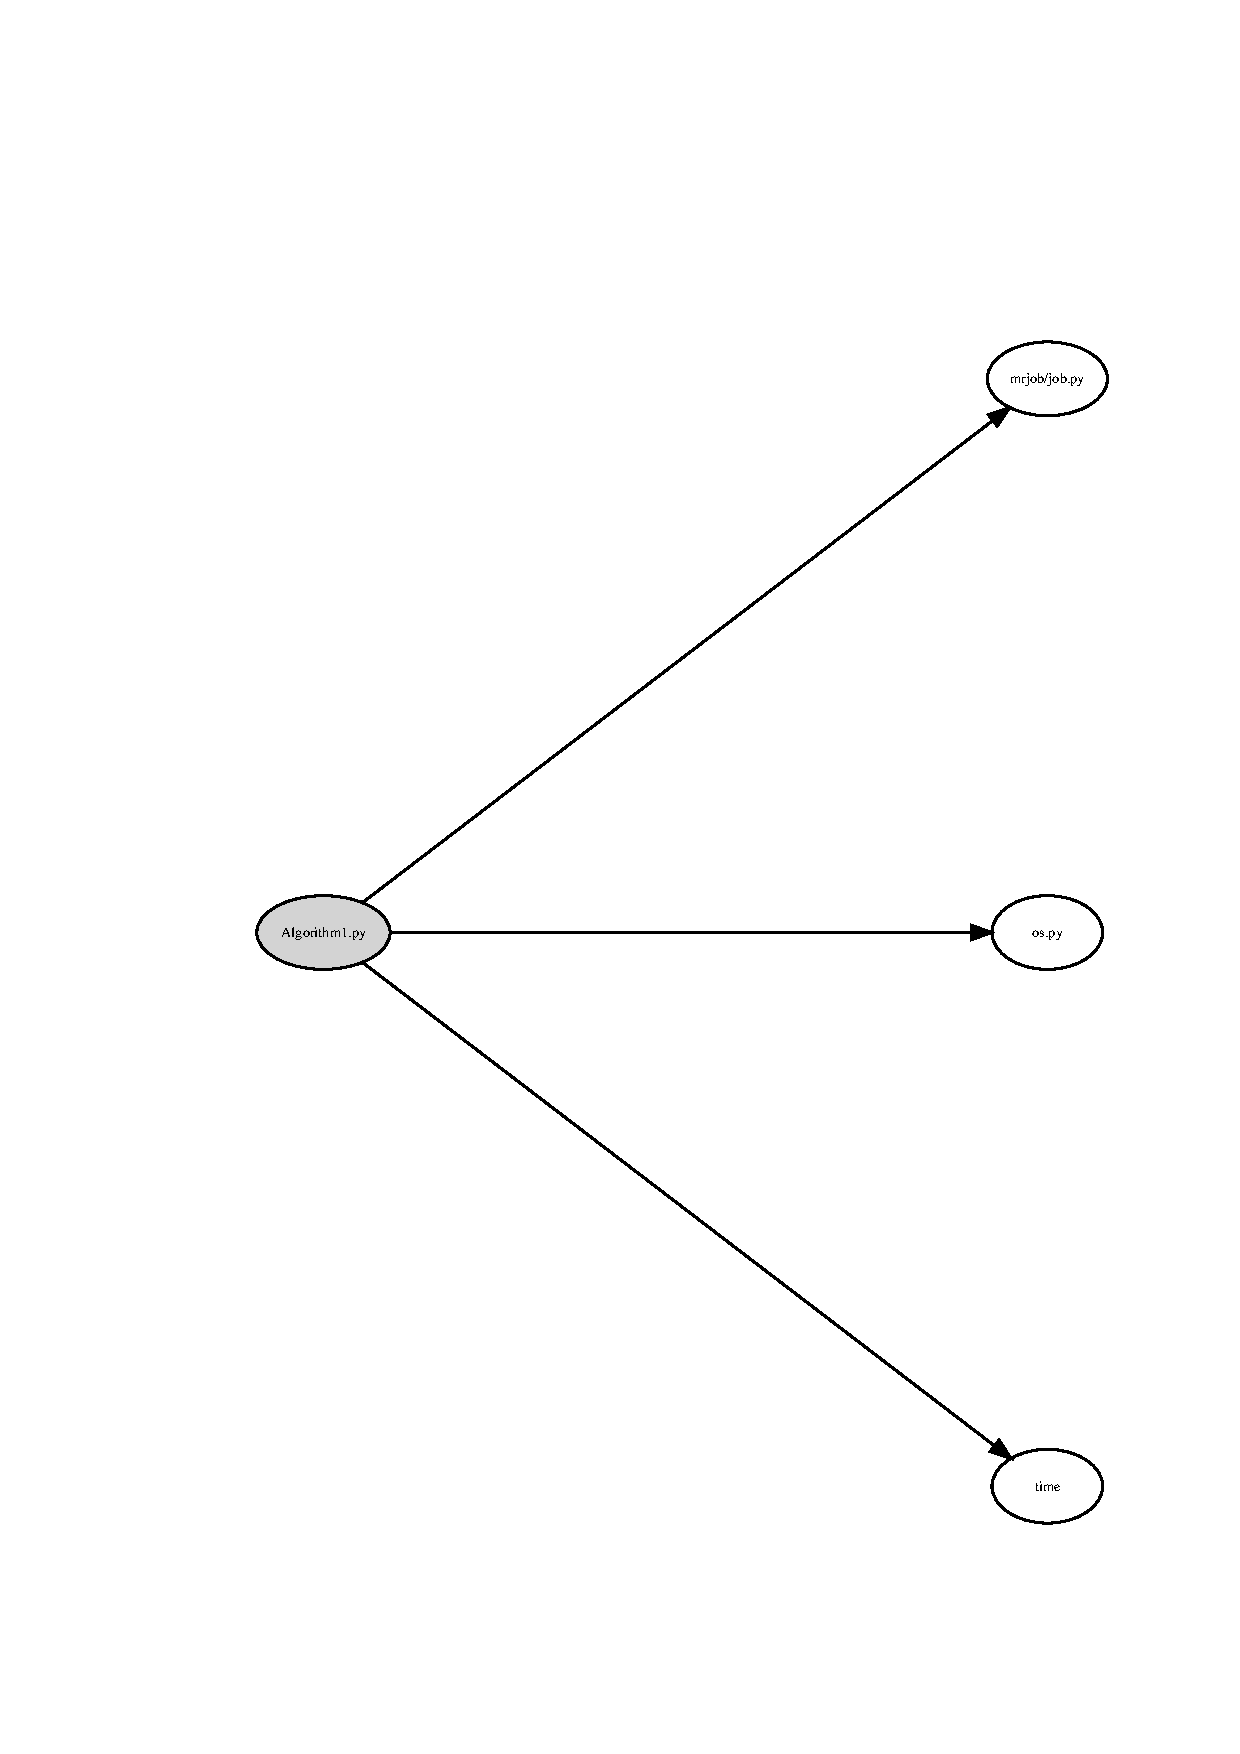
\includegraphics[width=\columnwidth]{Algo1}
 \centering 
  \caption {Dependency Diagram. }
 \end{figure}

This proves that the dependency metric behaves as it should. 




\subsection{Freevo Code Base Analysis} 
\noindent
What follows is the analysis using the chosen metrics of three major releases of the Freevo Media Center application. For each metric a summary output is given and any interesting points are elaborated upon. 

\subsubsection{Cyclomatic Complexity}

\paragraph{Freevo 1.7}
\noindent
The average cyclomatic complexity of all the methods/classes and functions in all of the python files in the source code is 4.0219. This is, according to \cite{mcCabe} a very good cyclomatic complexity. This average result however is extremely misleading as upon further inspection there are 73 methods/functions/classes with a cyclomatic complexity above 21 and 30 with a cyclomatic complexity of above 31 which is as Radon defines it alarmingly high and needs attention. There is one function that has a cyclomatic complexity of 102 which is unreasonably high and is most likely causing a number of bugs. This is the menu widget event handler method within the menu.py file. \\ 

\paragraph{Freevo 1.8}
\noindent
The average cyclomatic complexity of all the methods/classes and functions in all of the python files in the source code is 3.805. Which again is an extremely good score when it comes to cyclomatic complexity. It seems at a glance that the complexity has decreased which is counter-intuitive. However as before there are many classes/methods/functions with very high complexities. There are 94 classes/methods/functions with a cyclomatic complexity of higher than 21 and 39 classes/methods/functions with a cyclomatic complexity of higher than 31. The highest is once again the menu widget event handler method which has gone from a cyclomatic complexity of 102 to 116. 

\paragraph{Freevo 1.9}
\noindent
The average cyclomatic complexity of all the methods/classes and functions in all of the python files in the source code is 3.630. Yet again it appears that the cyclomatic complexity overall has decreased which implies good coding and significant effort was put in to make sure the complexity was well managed however as is the case for the previous two releases this result is misleading. There are 121 classes/methods/functions with a cylomatic complexity of higher than 21 and there are 48 methods/classes/functions with a cyclomatic complexity of higher than 31. Once again both of these numbers have increased quite significantly. One noteworthy piece of information is that the menu widget event handler method has decreased significantly from 116 to 55. \\

\noindent
A graph showing  both the number of very high error prone unstable blocks (i.e. cyclomatic complexity of higher than 21 (D) and 31 (E)) over the three releases along with the misleading average cyclomatic complexity can be seen in figure 2 below.



 \begin{figure}[H]
 \centering 
 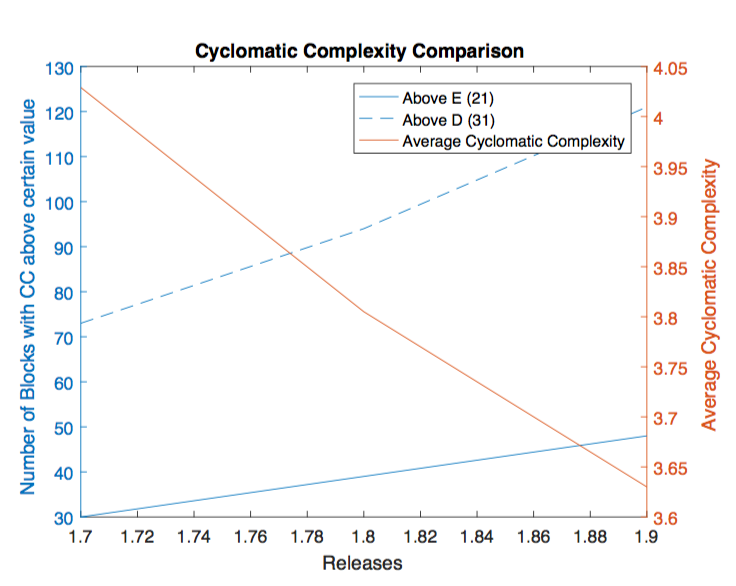
\includegraphics[width=\columnwidth]{CCcomp}
 \centering 
  \caption {Cyclomatic Complexity Graph. }
 \end{figure}

\noindent
 This graph indicates that while average cyclomatic complexity may be a tempting metric to use it does not give a good idea about the actual complexity of the program until you investigate each class, method and function individually. 




\subsubsection{Maintainability Index}

\paragraph{Freevo 1.7}


\paragraph{Freevo 1.8}


\paragraph{Freevo 1.8}



\subsubsection{Coverage}

\paragraph{Freevo 1.7}


\paragraph{Freevo 1.8}


\paragraph{Freevo 1.8}





\subsubsection{Halstead Effort and Difficulty Metrics}

\paragraph{Freevo 1.7}


\paragraph{Freevo 1.8}


\paragraph{Freevo 1.8}



\subsubsection{Dependencies}
\noindent
Shown in the figures 3-5 below are dependency graphs generated by Snakefood that show how the different files that make up each release of Freevo depend on each other and on external libraries. These graphs are extremely saturated and therefore a high level analysis approach is taken. These graphs are also included in the Appendix on a larger scale. 


\paragraph{Freevo 1.7}
\noindent

The dependency graph for Freevo 1.7 is shown in figure 3.

\begin{figure}[H]
 \centering 
 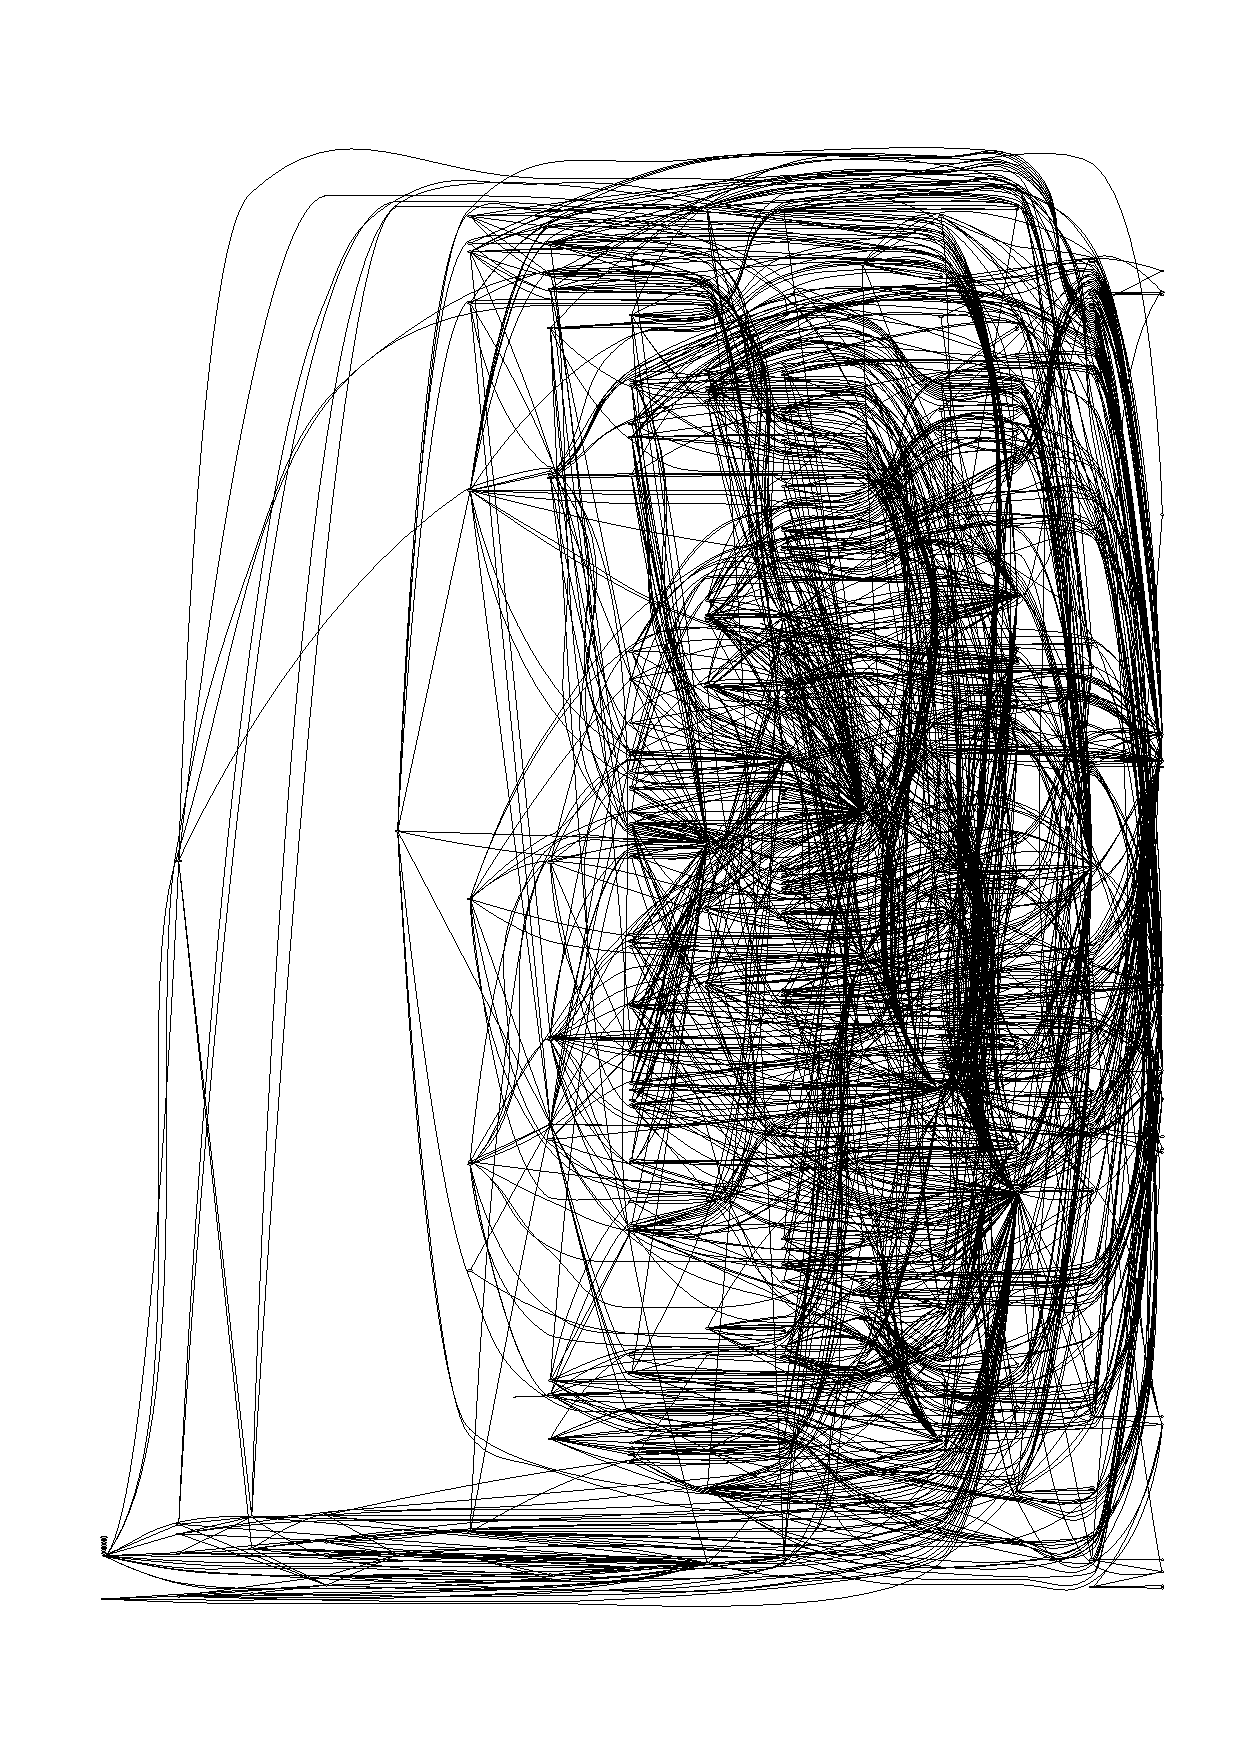
\includegraphics[width=\columnwidth]{17Full}
 \centering 
  \caption {Dependency Graph. }
 \end{figure}


\paragraph{Freevo 1.8}
\noindent
The dependency graph for Freevo 1.8 is shown in figure 4.

\begin{figure}[H]
 \centering 
 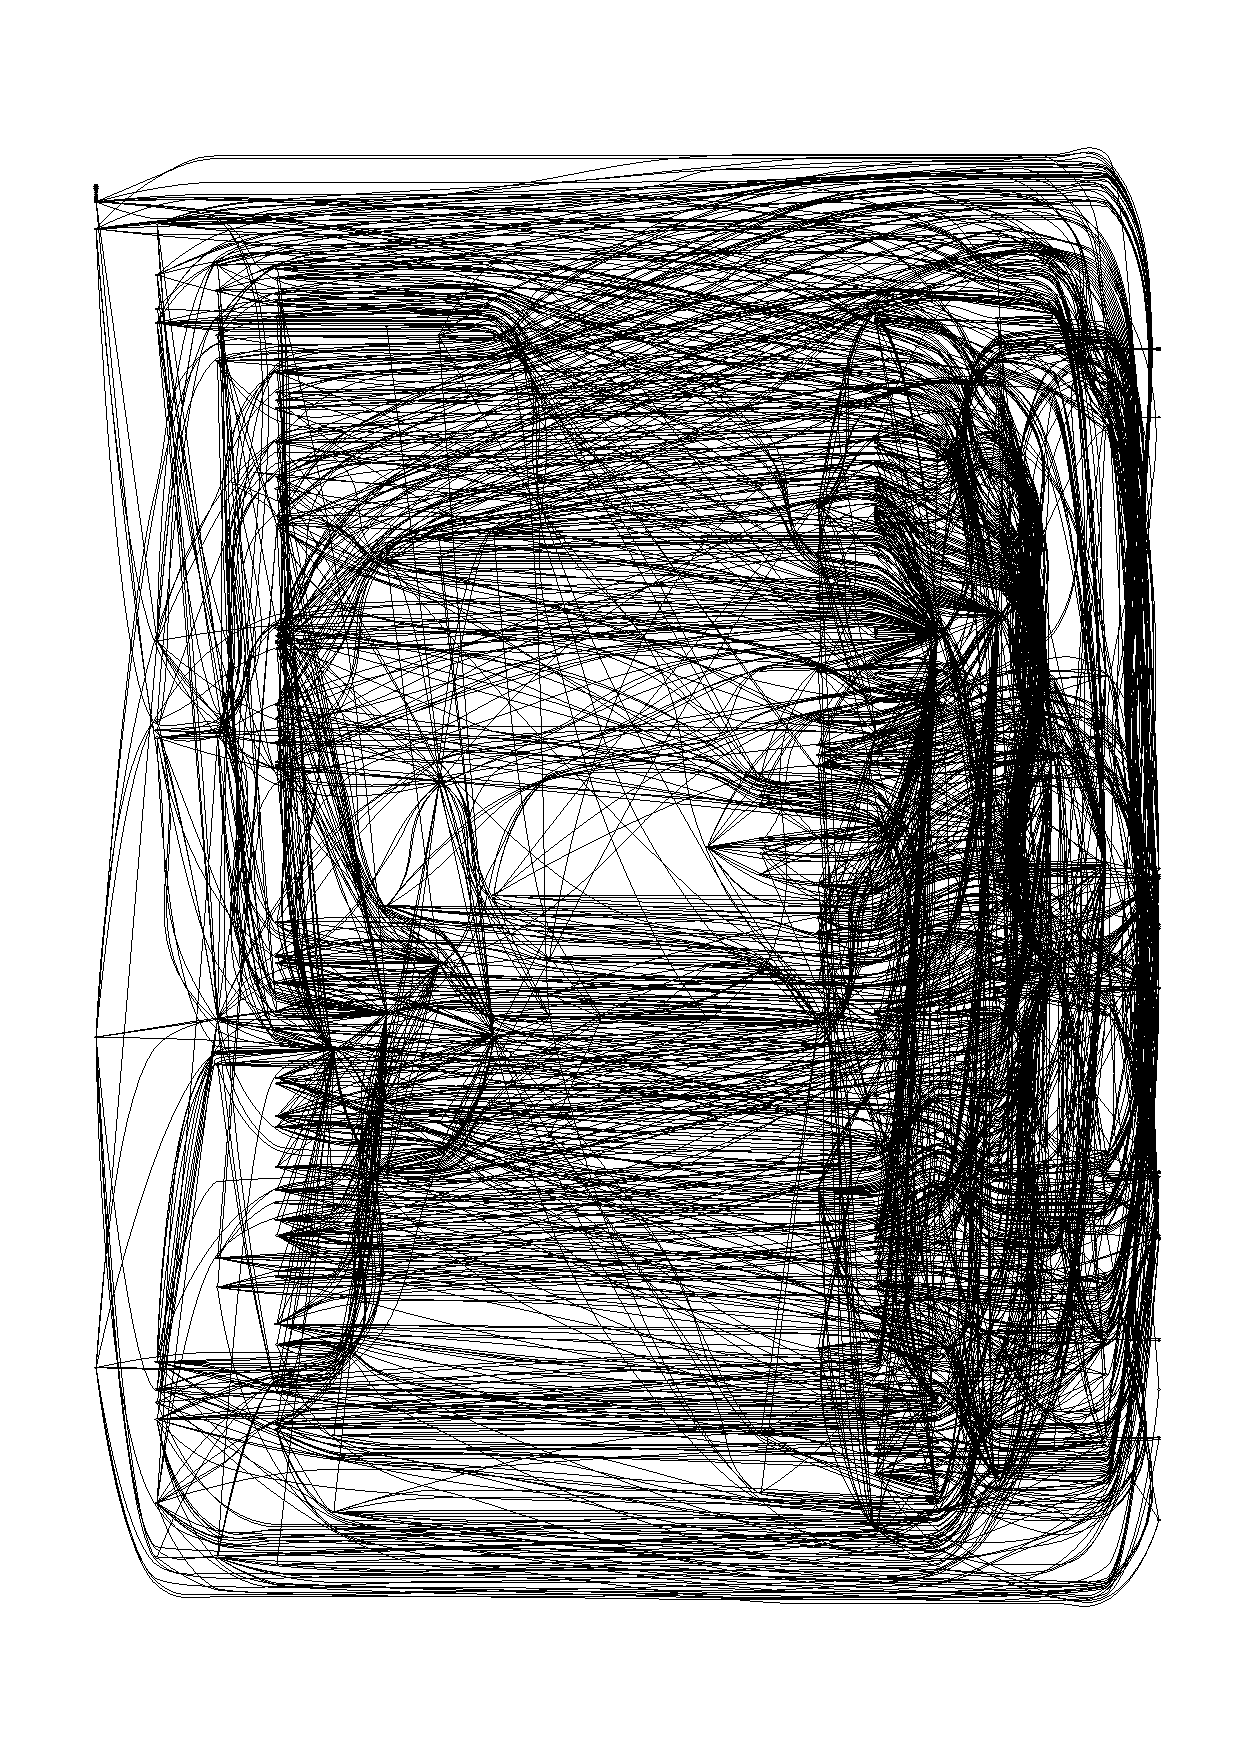
\includegraphics[width=\columnwidth]{18full}
 \centering 
  \caption {Dependency Graph. }
 \end{figure}



\paragraph{Freevo 1.9}
\noindent
The dependency graph for Freevo 1.9 is shown in figure 5.

\begin{figure}[]
 \centering 
 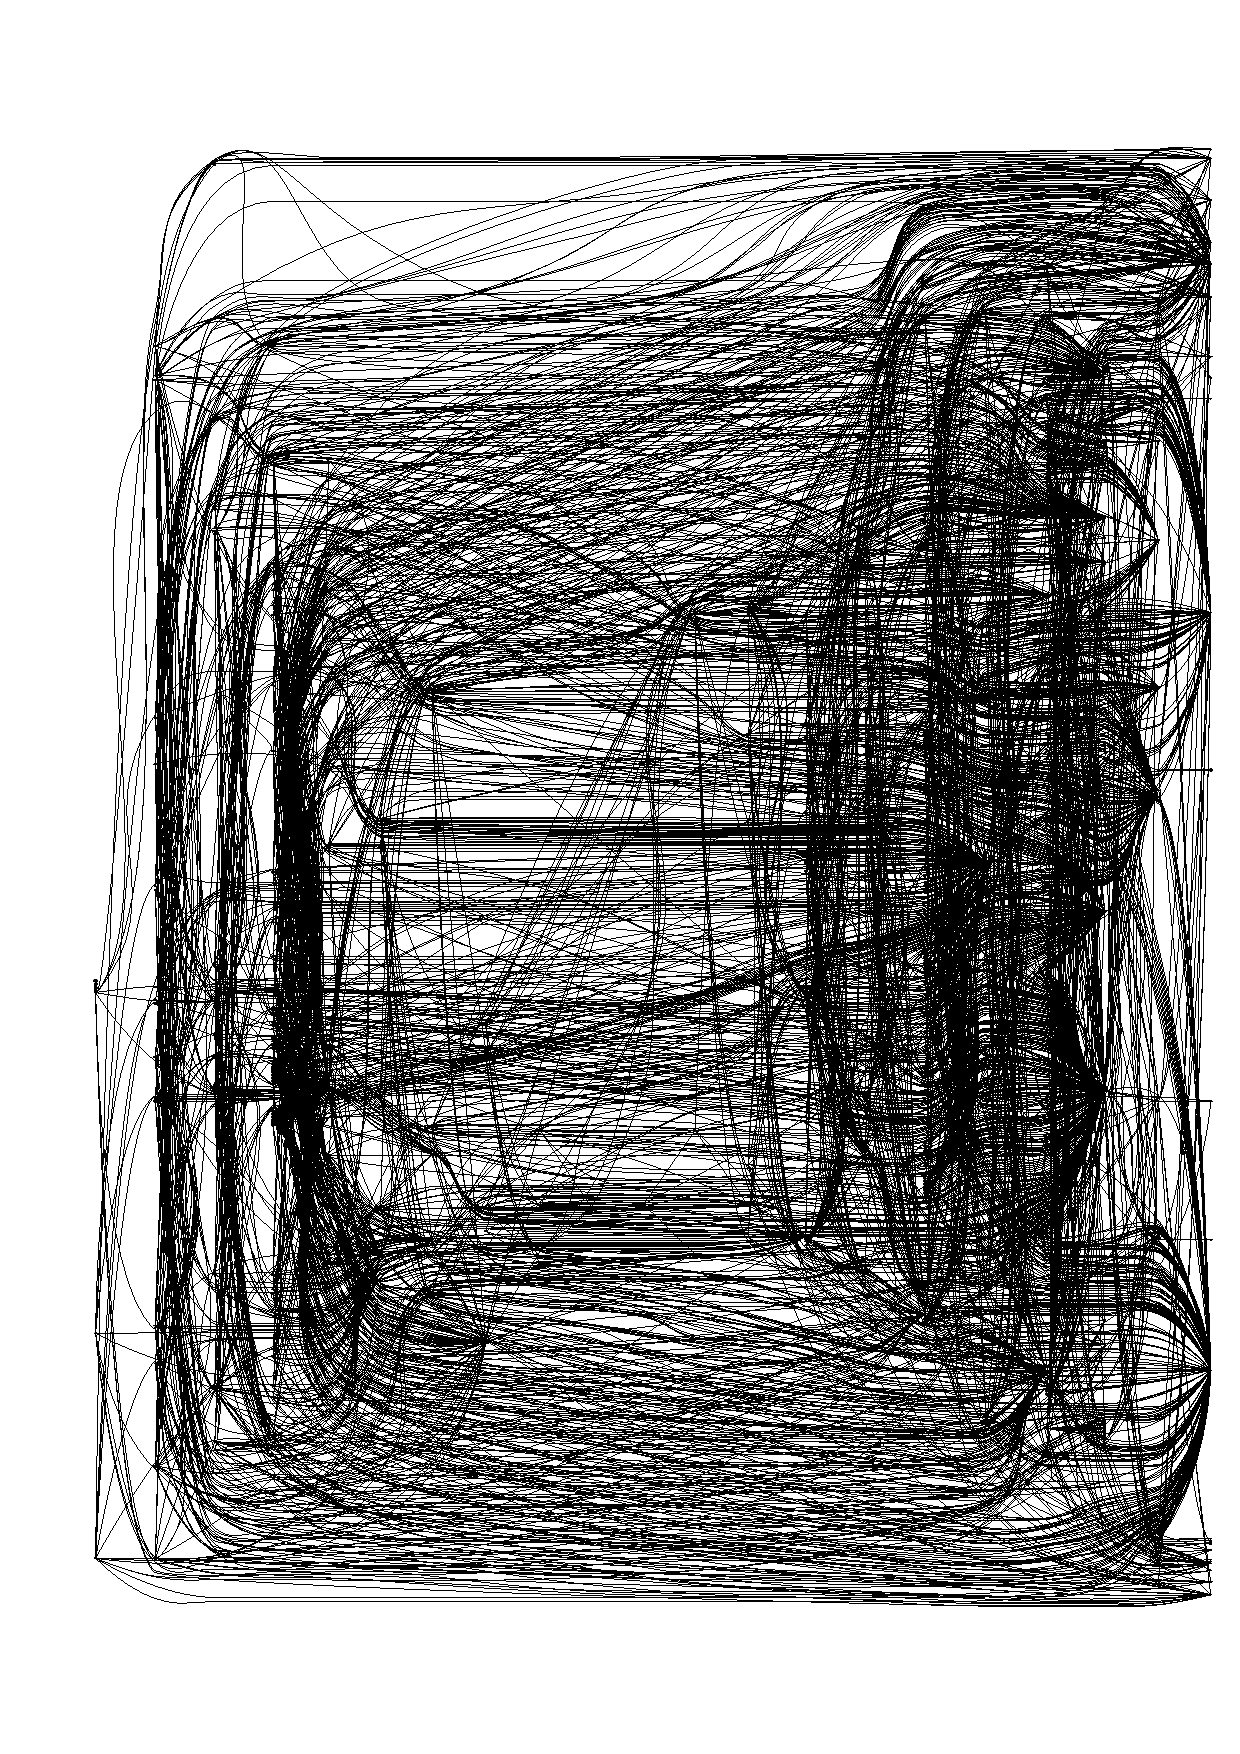
\includegraphics[width=\columnwidth]{19Full}
 \centering 
  \caption {Dependency Graph. }
 \end{figure}
 
 
 
 
 
 
\paragraph{Freevo 1.7 Without Follow}
\noindent

The dependency graph for Freevo 1.7 is shown in figure 3.

\begin{figure}[H]
 \centering 
 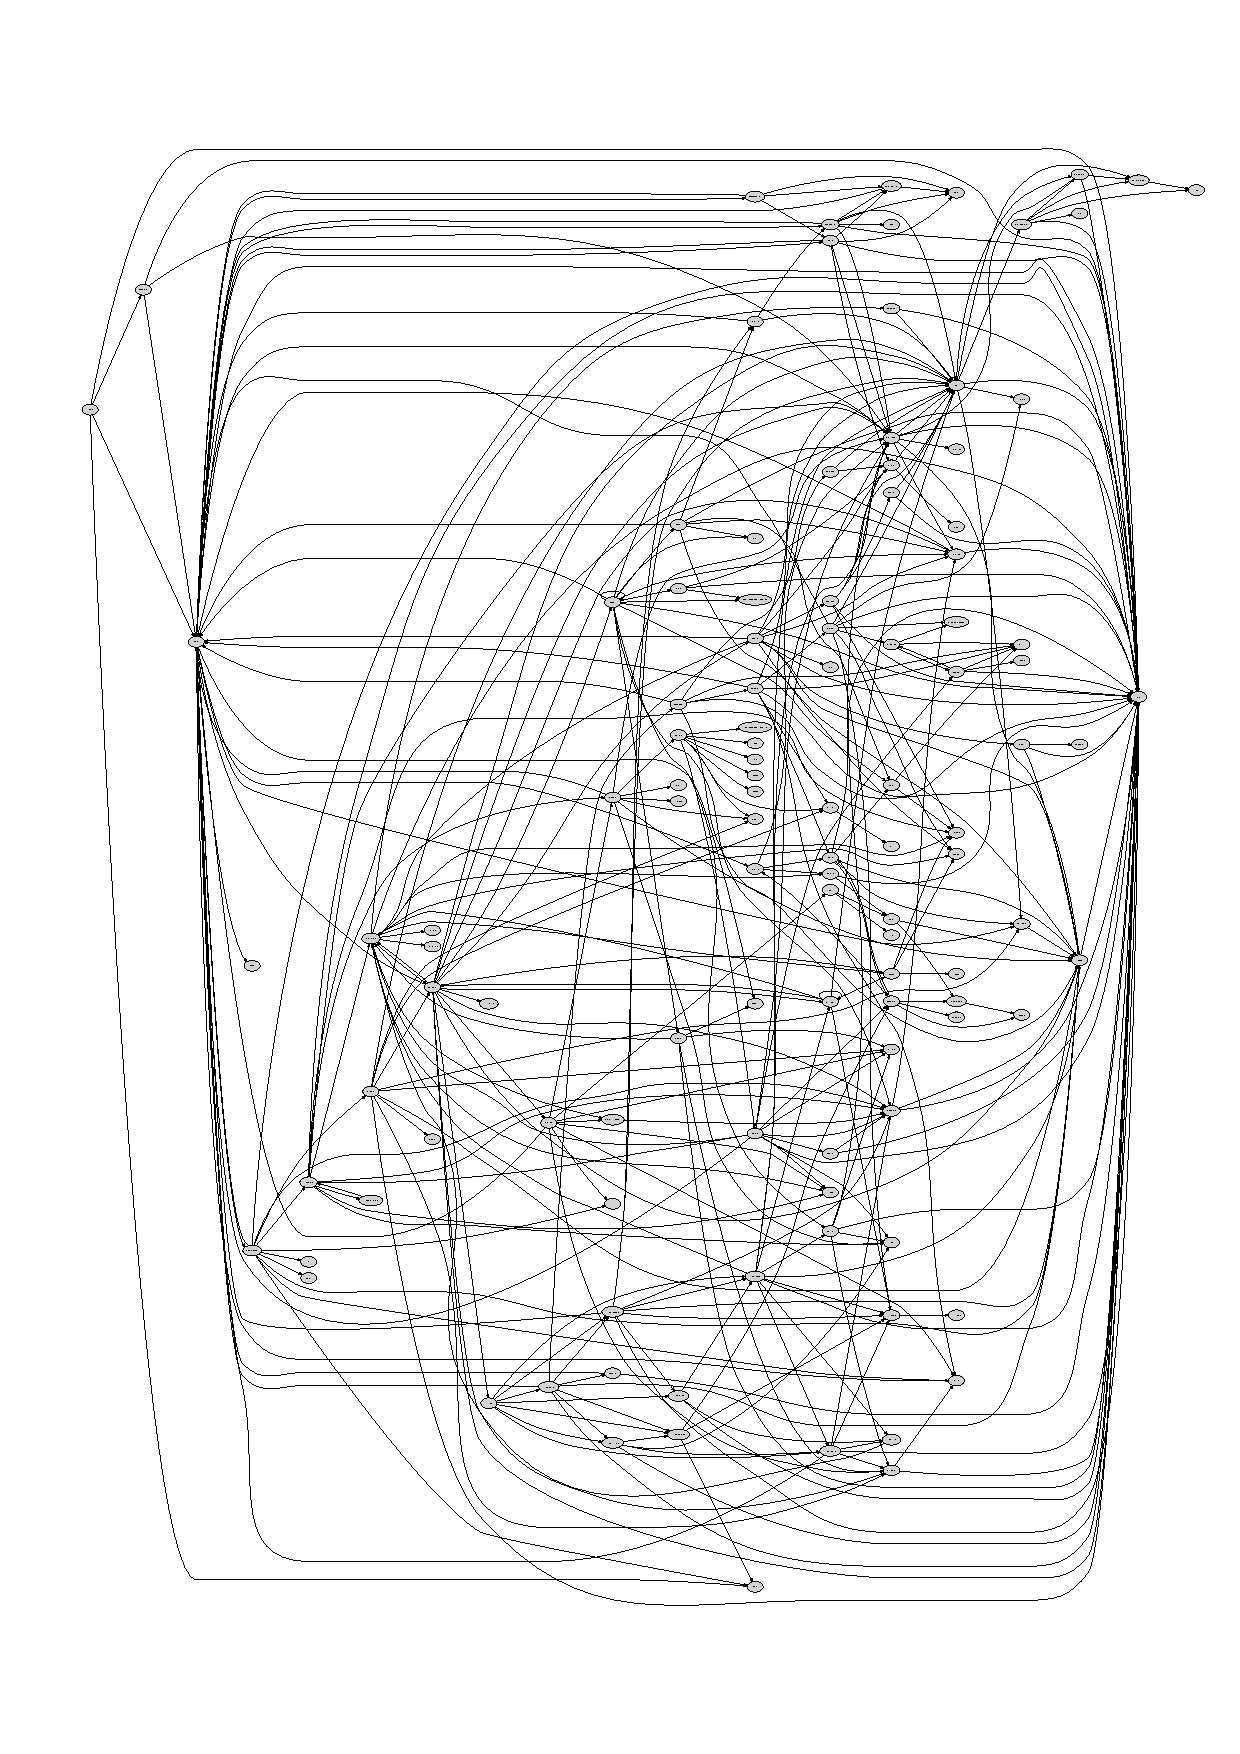
\includegraphics[width=\columnwidth]{freevo17less}
 \centering 
  \caption {Dependency Graph. }
 \end{figure}


\paragraph{Freevo 1.8 Without Follow}
\noindent
The dependency graph for Freevo 1.8 is shown in figure 4.

\begin{figure}[H]
 \centering 
 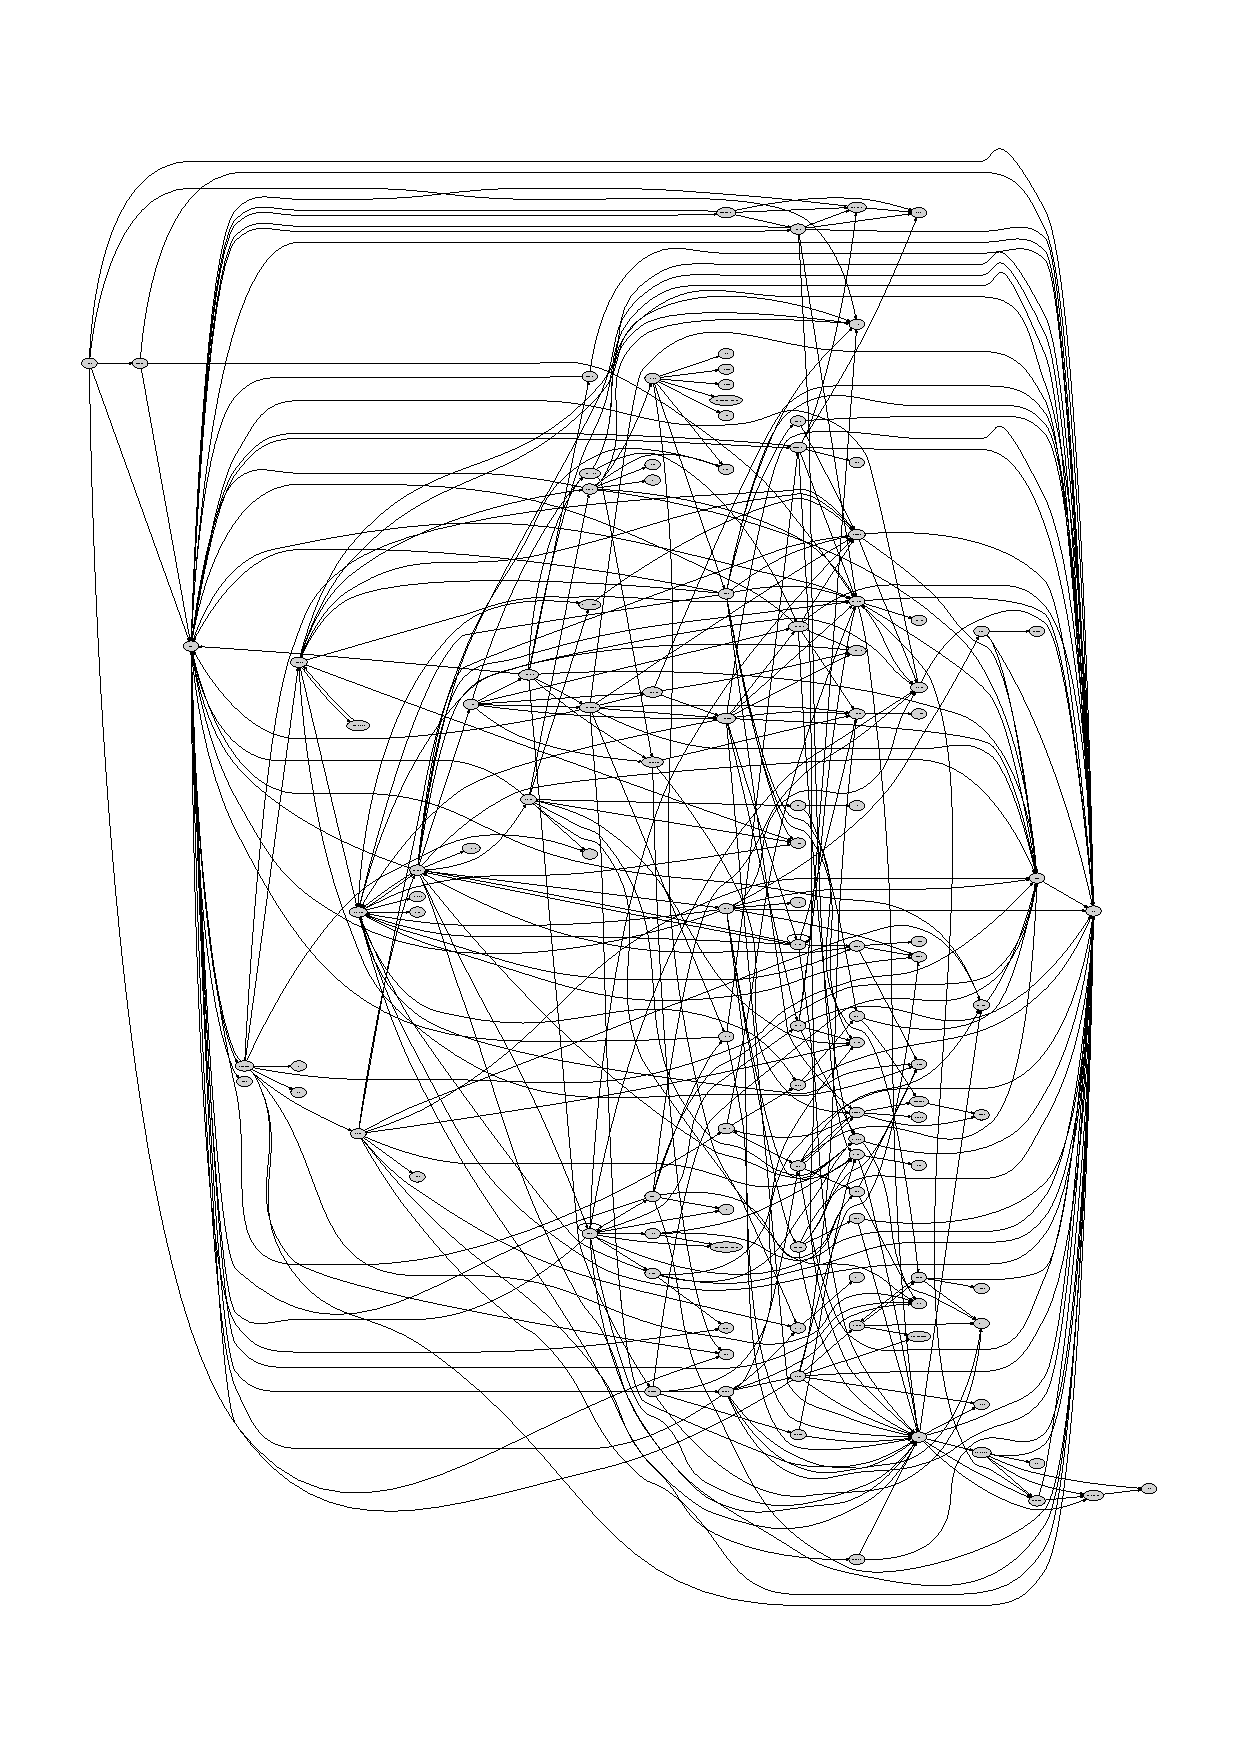
\includegraphics[width=\columnwidth]{freevo18less}
 \centering 
  \caption {Dependency Graph. }
 \end{figure}



\paragraph{Freevo 1.9 Without Follow}
\noindent
The dependency graph for Freevo 1.9 is shown in figure 5.

\begin{figure}[]
 \centering 
 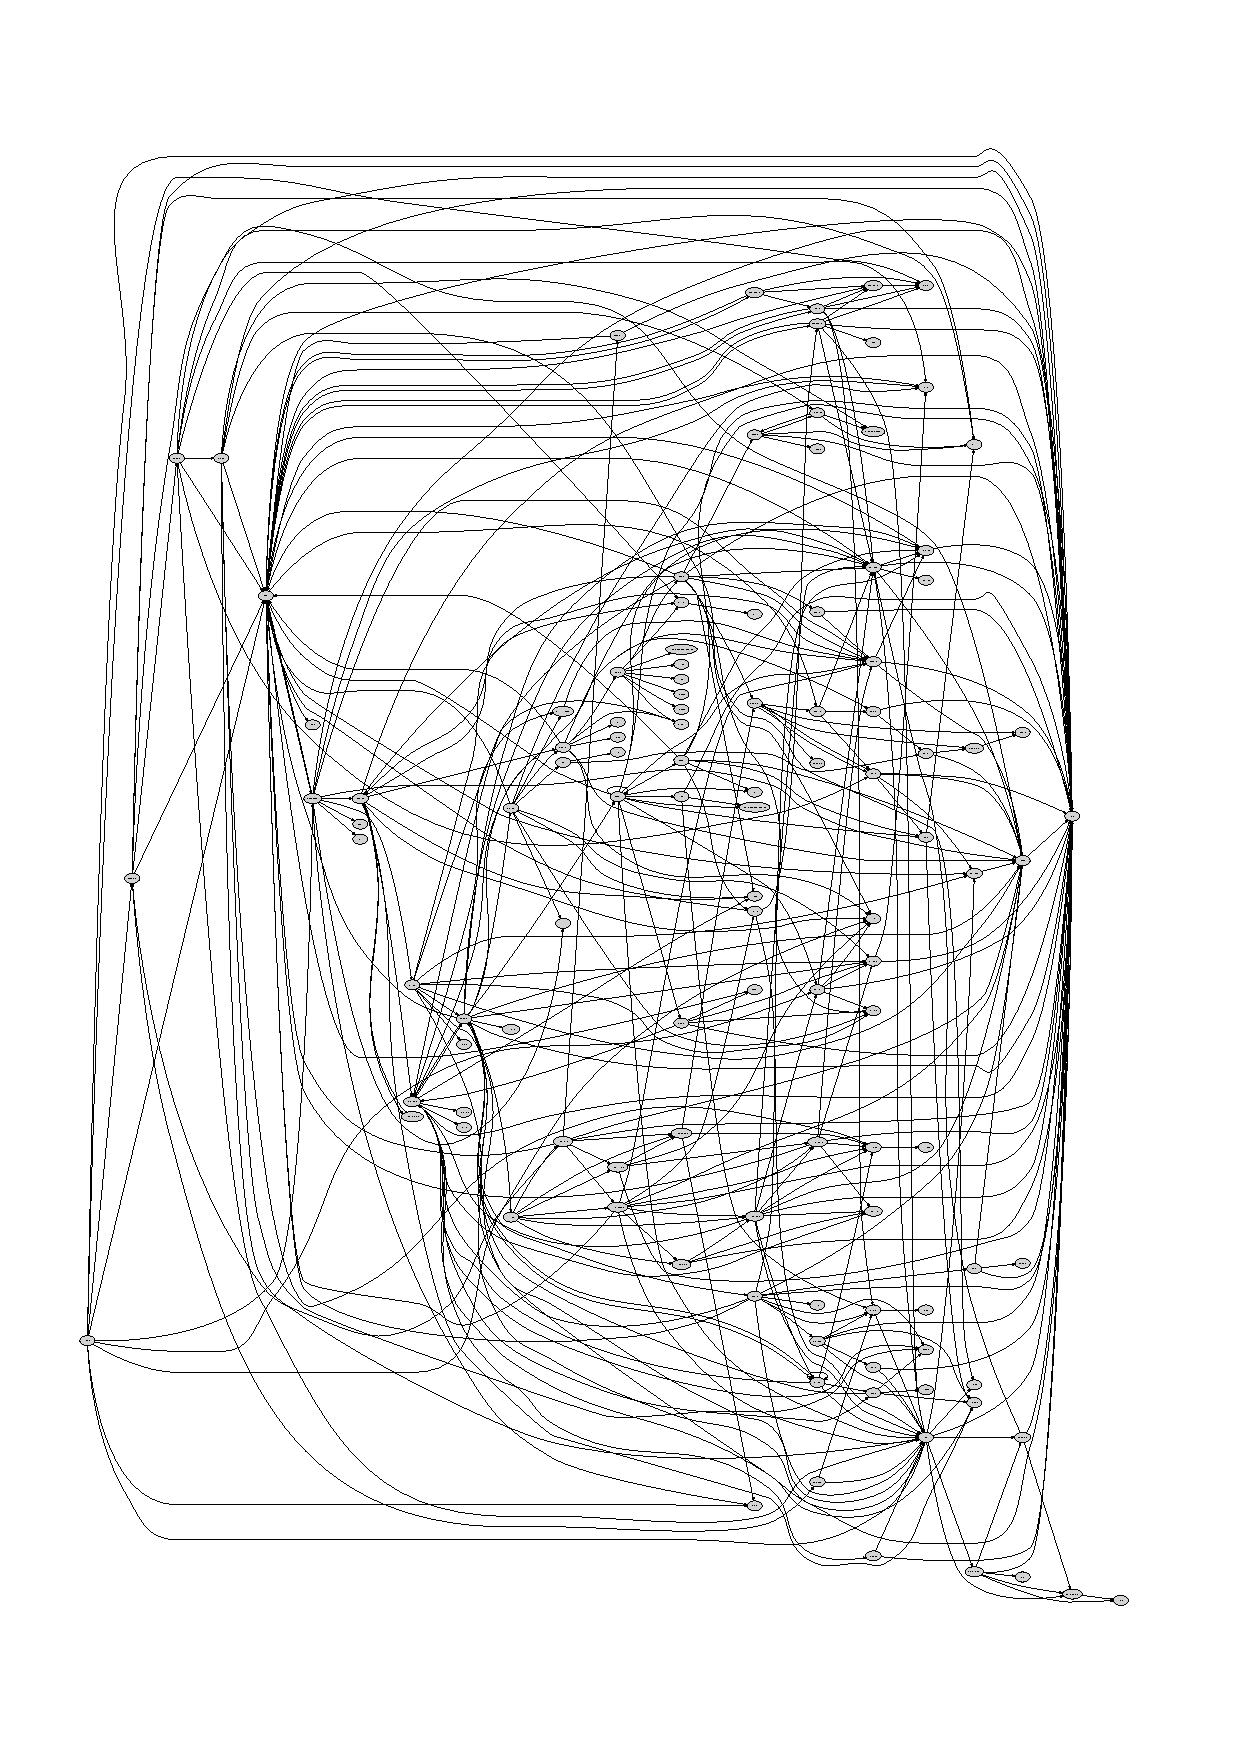
\includegraphics[width=\columnwidth]{freevo19less}
 \centering 
  \caption {Dependency Graph. }
 \end{figure}



\section{Additional Points of Interest}



\section{Conclusion}

% \begin{figure}[H]
% \centering 
% \includegraphics[width=\columnwidth]{warehouse1}
% \centering 
%  \caption {Lighting design for Sasol wax warehouse storage area using first set of lights }
% \end{figure}




\begin{thebibliography}{5}


  
\bibitem{mcCabe} Thomas J. McCabe, "A Complexity Measure". IEEE Transactions on Software Engineering, Vol. SE-2, No.4, December 1976. \\


\bibitem{MI1} Don Coleman, Dan Ash, Bruce Lowther, Paul Oman, "Using Metrics to Evaluate Software System Maintainability". Computing Practices, August 1994. \\




\bibitem{Linux} Lawrence Gray Thomas, "An Analysis of Software Quality and Maintainability Metrics with an Application to a Longitudinal Sudy of the Linux Kernel". Dissertation Submitted to the Faculty of the Graduate School of Vanderbilt University in partial fulfillment of the requirements for the degree of
Doctor of Philosophy in Computer Science, August, 2008.\\




\bibitem{HALS} Rafa E. Al Qutaish, Alain Abran, "An Analysis of the Design and Definitions of Halstead’s Metrics". Proceedings of the 15th International Workshop on Software Measurement, September 12-14, 2005, Montreal, Canada. pp. 337-352. \\

\bibitem{SPAG} Marwen Abbes, Foutse Khomh, Yann-Gaël Guéhéneuc, Giuliano Antoniol, "An Empirical Study of the Impact of Two Antipatterns, Blob and Spaghetti Code, On Program Comprehension". 15th European Conference on Software Maintenance and Reengineering, 2011. \\

\bibitem{Freevo} Dischi, "Freevo Website".\\
 \url{http://www.freevo.org}.
Last Accessed 18 April 2018. 


\end{thebibliography}

\onecolumn
\appendix


\lstinputlisting[caption=Author's code base to validate metric generation tools. ,language=python,numbers=left]{Algorithm1.py}





	% This is how you define a table: the [!hbt] means that LaTeX is forced (by the !) to place the table exactly here (by h), or if that doesnt work because of a pagebreak or so, it tries to place the table to the bottom of the page (by b) or the top (by t).


	% If you have questions about how to write mathematical formulas in LaTeX, please read a LaTeX book or the 'Not So Short Introduction to LaTeX': tobi.oetiker.ch/lshort/lshort.pdf

% Now we need a bibliography:


% Your document ends here!
\end{document}